\documentclass[pdflatex,sn-mathphys-num]{sn-jnl}

\usepackage{graphicx}
\usepackage{amsmath,amssymb,amsfonts}
\usepackage{booktabs}
\usepackage{tabularx}
\usepackage{hyperref}
\hypersetup{hypertexnames=false}

\raggedbottom

\begin{document}

\title[Standalone numerical study for the calibrated gDMR parameter set with positive rate]{Standalone numerical study for the calibrated gDMR parameter set with positive rate}

\author[1]{\fnm{Mara Kalicanin} \sur{Dimitrov}}
\author[1]{\fnm{Ying} \sur{Ni}}
\affil[1]{\orgdiv{Department of Business and Mathematics}, \orgname{M\"{a}lardalen University}, \orgaddress{\postcode{721~23}, \city{V\"{a}ster{\aa}s}, \country{Sweden}}}

\maketitle

\section{Numerical studies}

This standalone document repeats the manuscript numerical-study design for the calibrated gDMR parameter set reported in Table~\ref{tab:bgk_r02_calibrated_t1_nex12-experimental-setting}, using the positive risk-free rate \(r=0.02\). The option is a Bermudan put with twelve exercise dates, maturity \(T=1\), and strikes \(K=70,80,90,100,110\). The direct plain LSMC estimator is compared with the Hybrid LSMC--PDE estimator. All prices, standard errors, confidence intervals, and relative errors are computed from the direct estimators, and benchmark-relative errors use the plain LSMC references in Table~\ref{tab:bgk_r02_calibrated_t1_nex12-benchmark-references}.

\begin{table}[htbp]
\centering
\caption{Model and numerical parameters for the standalone calibrated positive-rate study.}
\label{tab:bgk_r02_calibrated_t1_nex12-experimental-setting}
\begin{tabular}{lr}
\toprule
Quantity & Value \\
\midrule
Model & gDMR \\
Option & Bermudan put \\
$S_0$ & 100.0 \\
$K$ & 70, 80, 90, 100, 110 \\
$T$ & 1.0 \\
$r$ & 0.02 \\
$v_0$ & 0.114 \\
$v'_0$ & 0.110 \\
$\kappa_1$ & 5.5 \\
$\kappa_2$ & 0.1 \\
$\theta$ & 0.078 \\
$\xi_1$ & 2.689 \\
$\xi_2$ & 0.502 \\
$\rho_{12}$ & -0.982 \\
$\rho_{13}$ & -0.727 \\
$\rho_{23}$ & 0.590 \\
$\delta_1$ & 0.94 \\
$\delta_2$ & 0.94 \\
Exercise dates & 12 \\
Benchmark & LSMC, 1200 steps, 1,200,000 paths \\
Hybrid asset grid & 301 \\
\bottomrule
\end{tabular}
\end{table}


The benchmark references are obtained with \(1200\) Euler time steps and \(1,200,000\) direct paths. Across the five strikes, the benchmark direct prices range from 2.522851 to 15.743520. These values define the reference scale used in the step-sweep and path-sweep experiments below.

\begin{table}[htbp]
\centering
\caption{Benchmark direct LSMC reference prices for the standalone study.}
\label{tab:bgk_r02_calibrated_t1_nex12-benchmark-references}
\begin{tabular}{rrrrr}
\toprule
Strike & Price & SE & CI lower & CI upper \\
\midrule
70 & 2.522851 & 0.007103 & 2.508929 & 2.536773 \\
80 & 4.298933 & 0.009345 & 4.280617 & 4.317249 \\
90 & 6.942119 & 0.011774 & 6.919042 & 6.965196 \\
100 & 10.682037 & 0.014105 & 10.654391 & 10.709683 \\
110 & 15.743520 & 0.015757 & 15.712636 & 15.774404 \\
\bottomrule
\end{tabular}
\end{table}


\subsection{Fixed path budget, varying number of Euler time steps}

The first experiment keeps the direct path budget fixed and varies the number of Euler time steps. The two path budgets are \(20,000\) and \(60,000\), and both methods are evaluated at \(24\), \(48\), \(72\), and \(96\) steps. This isolates how the time discretization affects the direct Bermudan estimator away from the benchmark regime.

For \(20,000\) paths, the LSMC relative-error range over the full step-sweep grid is 0.344\%--8.645\%, while the Hybrid LSMC--PDE range is 0.019\%--7.459\%. Figure~\ref{fig:bgk_r02_calibrated_t1_nex12-step20k} shows the strike-wise relative-error profiles, and Table~\ref{tab:bgk_r02_calibrated_t1_nex12-step72-20k} reports the representative \(72\)-step values.

\begin{figure}[htbp]
\centering
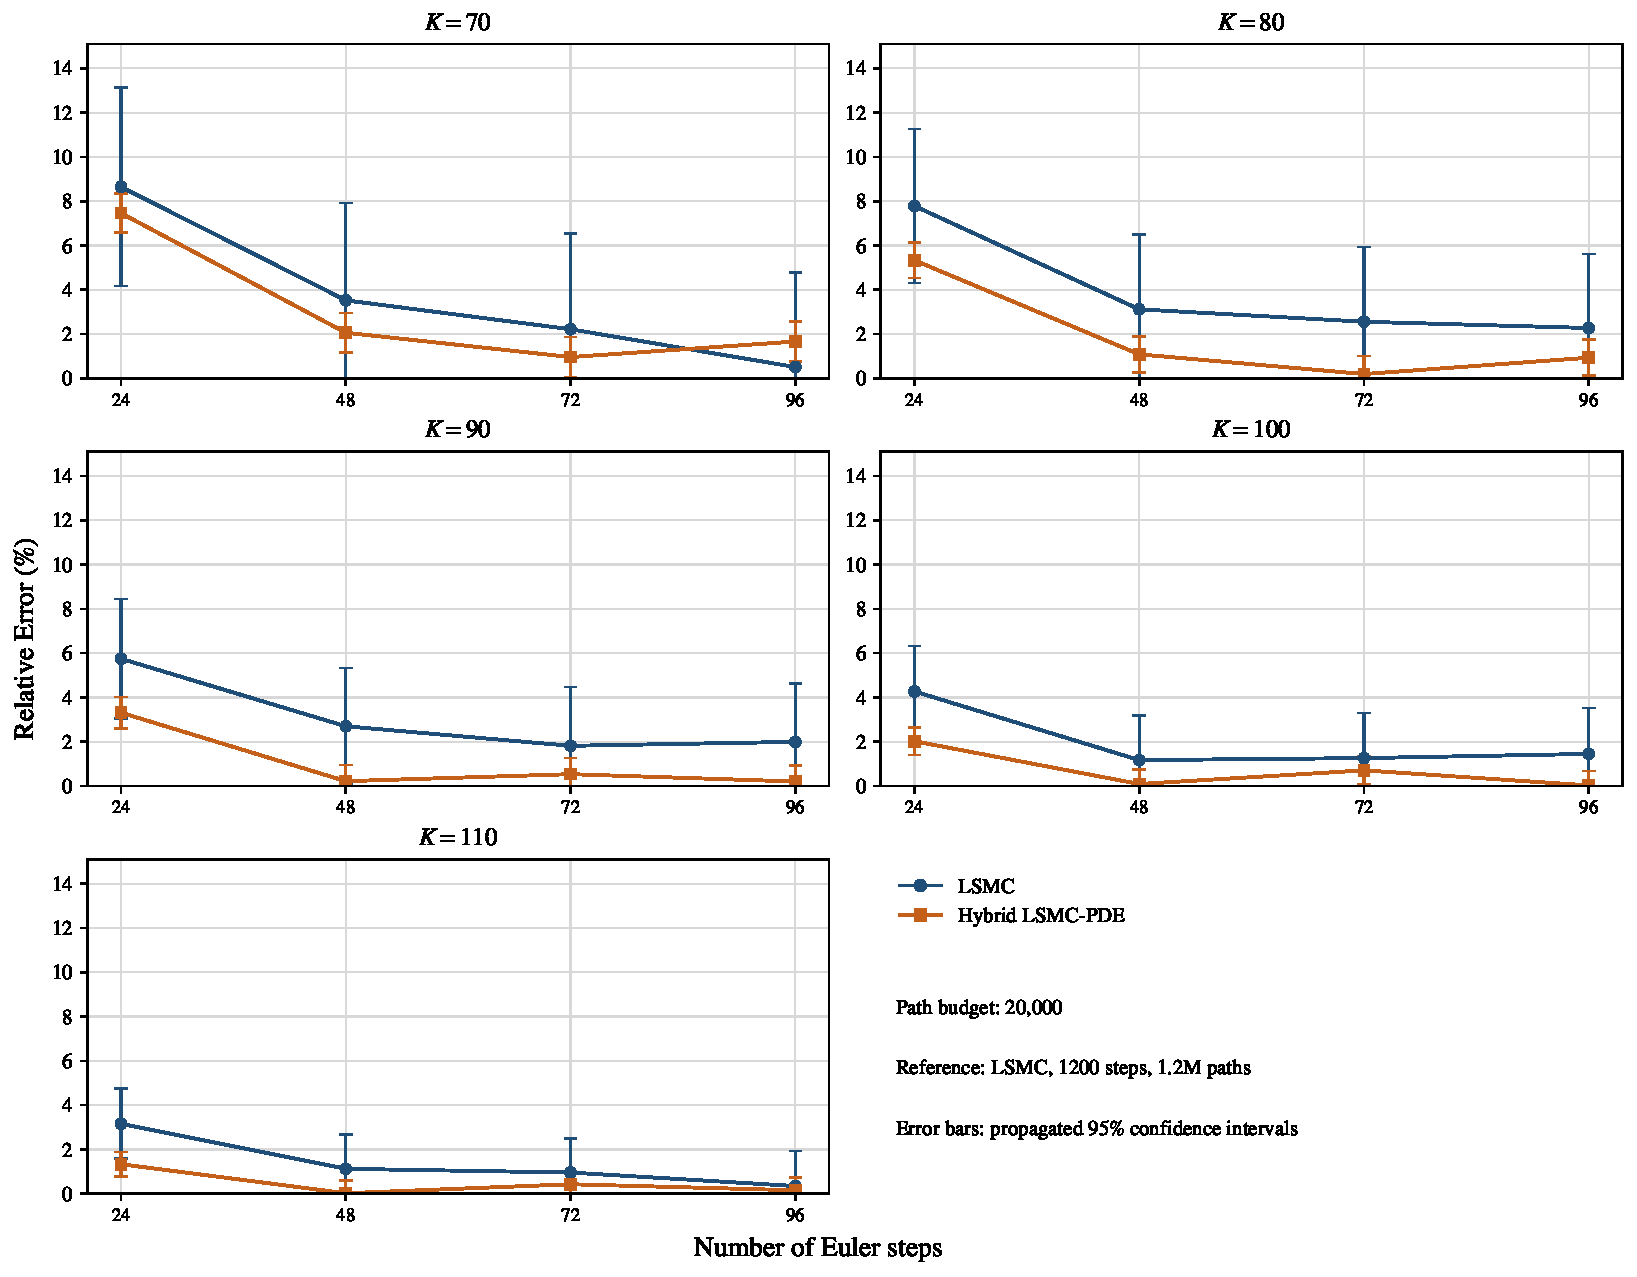
\includegraphics[width=0.96\textwidth]{../figures/bgk_r02_calibrated_t1_nex12_step_sweep_20k_direct_relative_error.pdf}
\caption{Relative errors for the matched \(20{,}000\)-path step-sweep experiment. Error bars are induced by the \(95\%\) confidence intervals of the direct estimators.}
\label{fig:bgk_r02_calibrated_t1_nex12-step20k}
\end{figure}

\begin{table}[htbp]
\centering
\caption{Representative direct metrics at 20,000 paths and 72 Euler steps.}
\label{tab:bgk_r02_calibrated_t1_nex12-step72-20k}
\begin{tabular}{lrrrr}
\toprule
Strike & LSMC price & LSMC rel. err. & Hybrid price & Hybrid rel. err. \\
\midrule
$70$ & 2.578706 & 2.214\% & 2.547003 & 0.957\% \\
$80$ & 4.408717 & 2.554\% & 4.307120 & 0.190\% \\
$90$ & 7.068072 & 1.814\% & 6.905102 & 0.533\% \\
$100$ & 10.816495 & 1.259\% & 10.606747 & 0.705\% \\
$110$ & 15.893853 & 0.955\% & 15.676443 & 0.426\% \\
\bottomrule
\end{tabular}
\end{table}


For \(60,000\) paths, the same design gives an LSMC relative-error range of 0.102\%--7.720\% and a Hybrid LSMC--PDE range of 0.028\%--7.857\%. Figure~\ref{fig:bgk_r02_calibrated_t1_nex12-step60k} and Table~\ref{tab:bgk_r02_calibrated_t1_nex12-step72-60k} give the corresponding graphical and tabular summaries.

\begin{figure}[htbp]
\centering
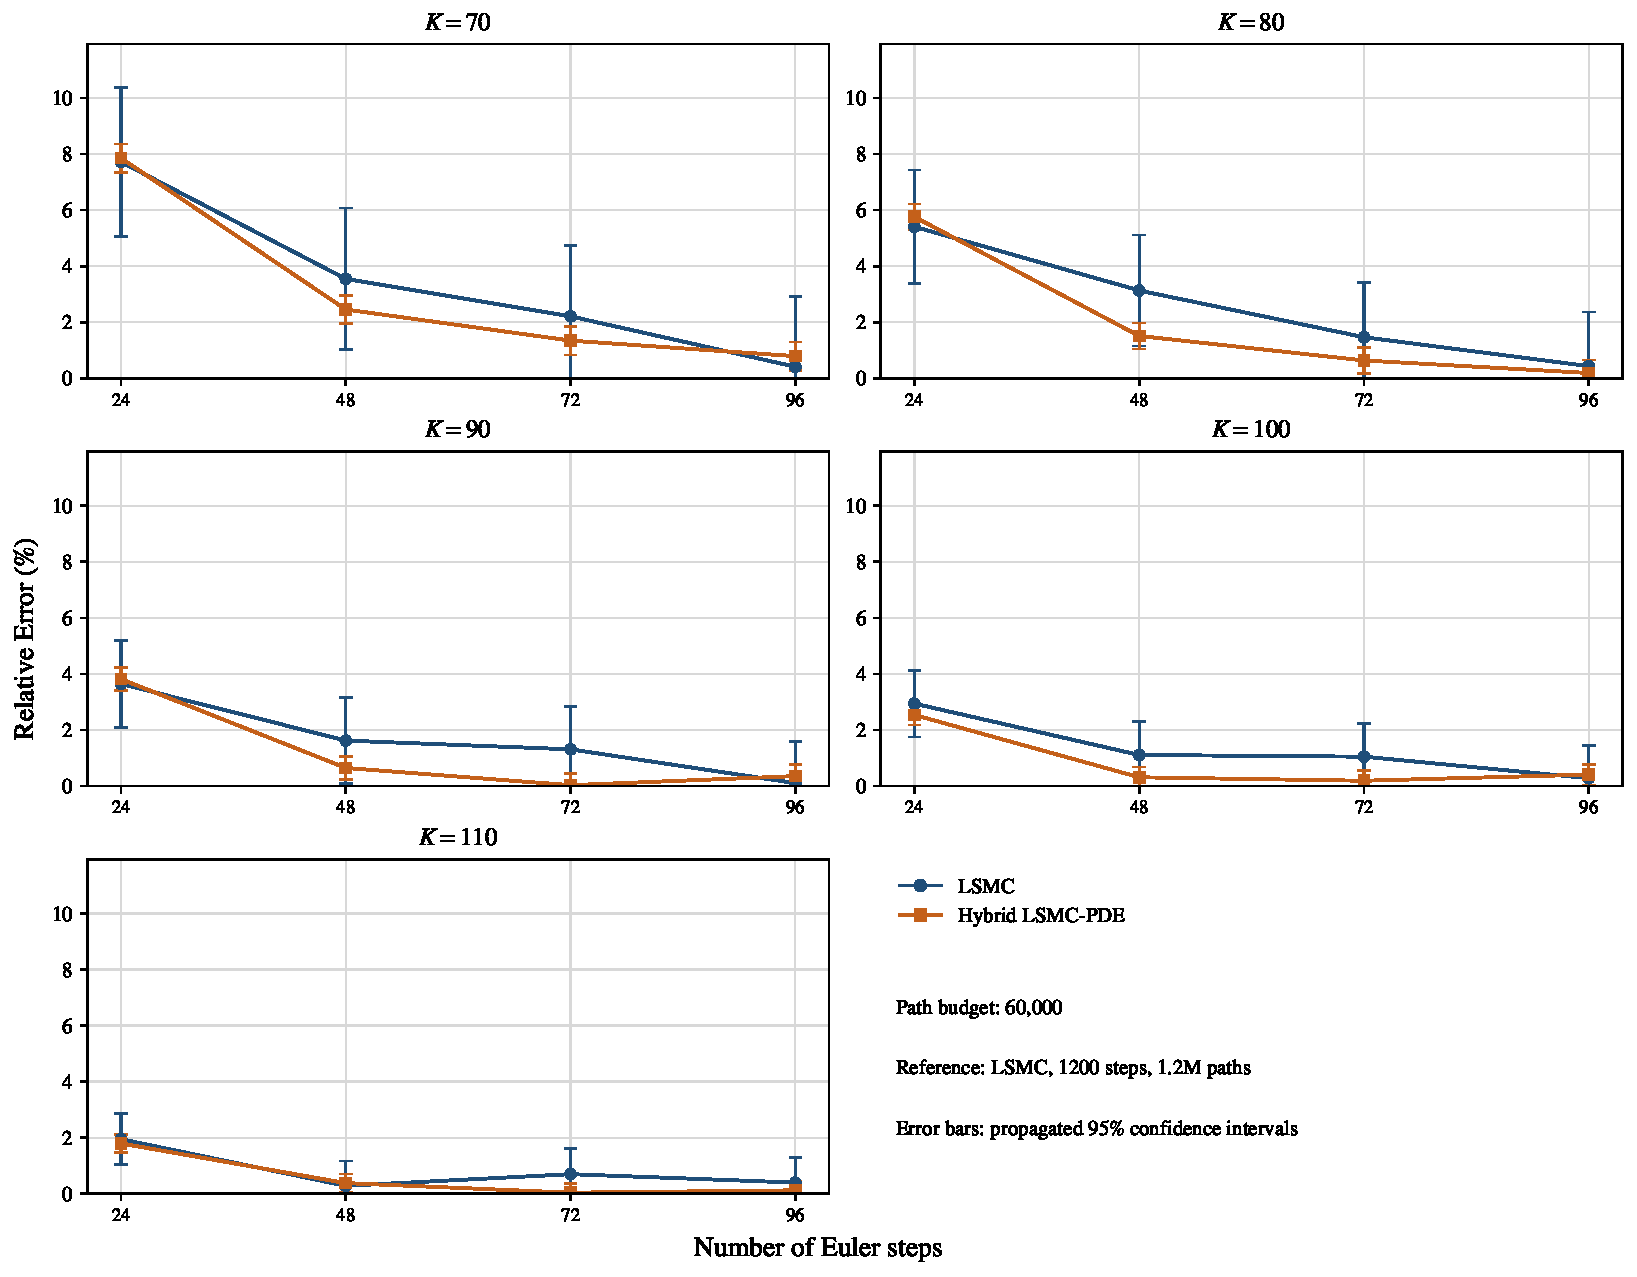
\includegraphics[width=0.96\textwidth]{../figures/bgk_r02_calibrated_t1_nex12_step_sweep_60k_direct_relative_error.pdf}
\caption{Relative errors for the matched \(60{,}000\)-path step-sweep experiment. Error bars are induced by the \(95\%\) confidence intervals of the direct estimators.}
\label{fig:bgk_r02_calibrated_t1_nex12-step60k}
\end{figure}

\begin{table}[htbp]
\centering
\caption{Representative direct metrics at 60,000 paths and 72 Euler steps.}
\label{tab:bgk_r02_calibrated_t1_nex12-step72-60k}
\begin{tabular}{lrrrr}
\toprule
Strike & LSMC price & LSMC rel. err. & Hybrid price & Hybrid rel. err. \\
\midrule
$70$ & 2.578570 & 2.209\% & 2.556746 & 1.344\% \\
$80$ & 4.361900 & 1.465\% & 4.326225 & 0.635\% \\
$90$ & 7.032832 & 1.307\% & 6.940184 & 0.028\% \\
$100$ & 10.793695 & 1.045\% & 10.662148 & 0.186\% \\
$110$ & 15.853083 & 0.696\% & 15.749100 & 0.035\% \\
\bottomrule
\end{tabular}
\end{table}


\subsection{Fixed number of Euler time steps, varying path counts}

The second experiment fixes the number of Euler time steps and varies the direct path budget. The reported path grid is \(250\), \(1000\), \(5000\), \(10000\), \(20000\), \(40000\), and \(60000\). The two discretization levels are \(48\) and \(60\) steps.

At \(48\) steps for the at-the-money strike, the LSMC relative-error range over all path counts is 1.105\%--25.948\%, while the Hybrid LSMC--PDE range is 0.088\%--11.118\%. Figure~\ref{fig:bgk_r02_calibrated_t1_nex12-path48} reports the full strike-wise path sweep, and Table~\ref{tab:bgk_r02_calibrated_t1_nex12-path48-path20k} reports the \(20,000\)-path representative values.

\begin{figure}[htbp]
\centering
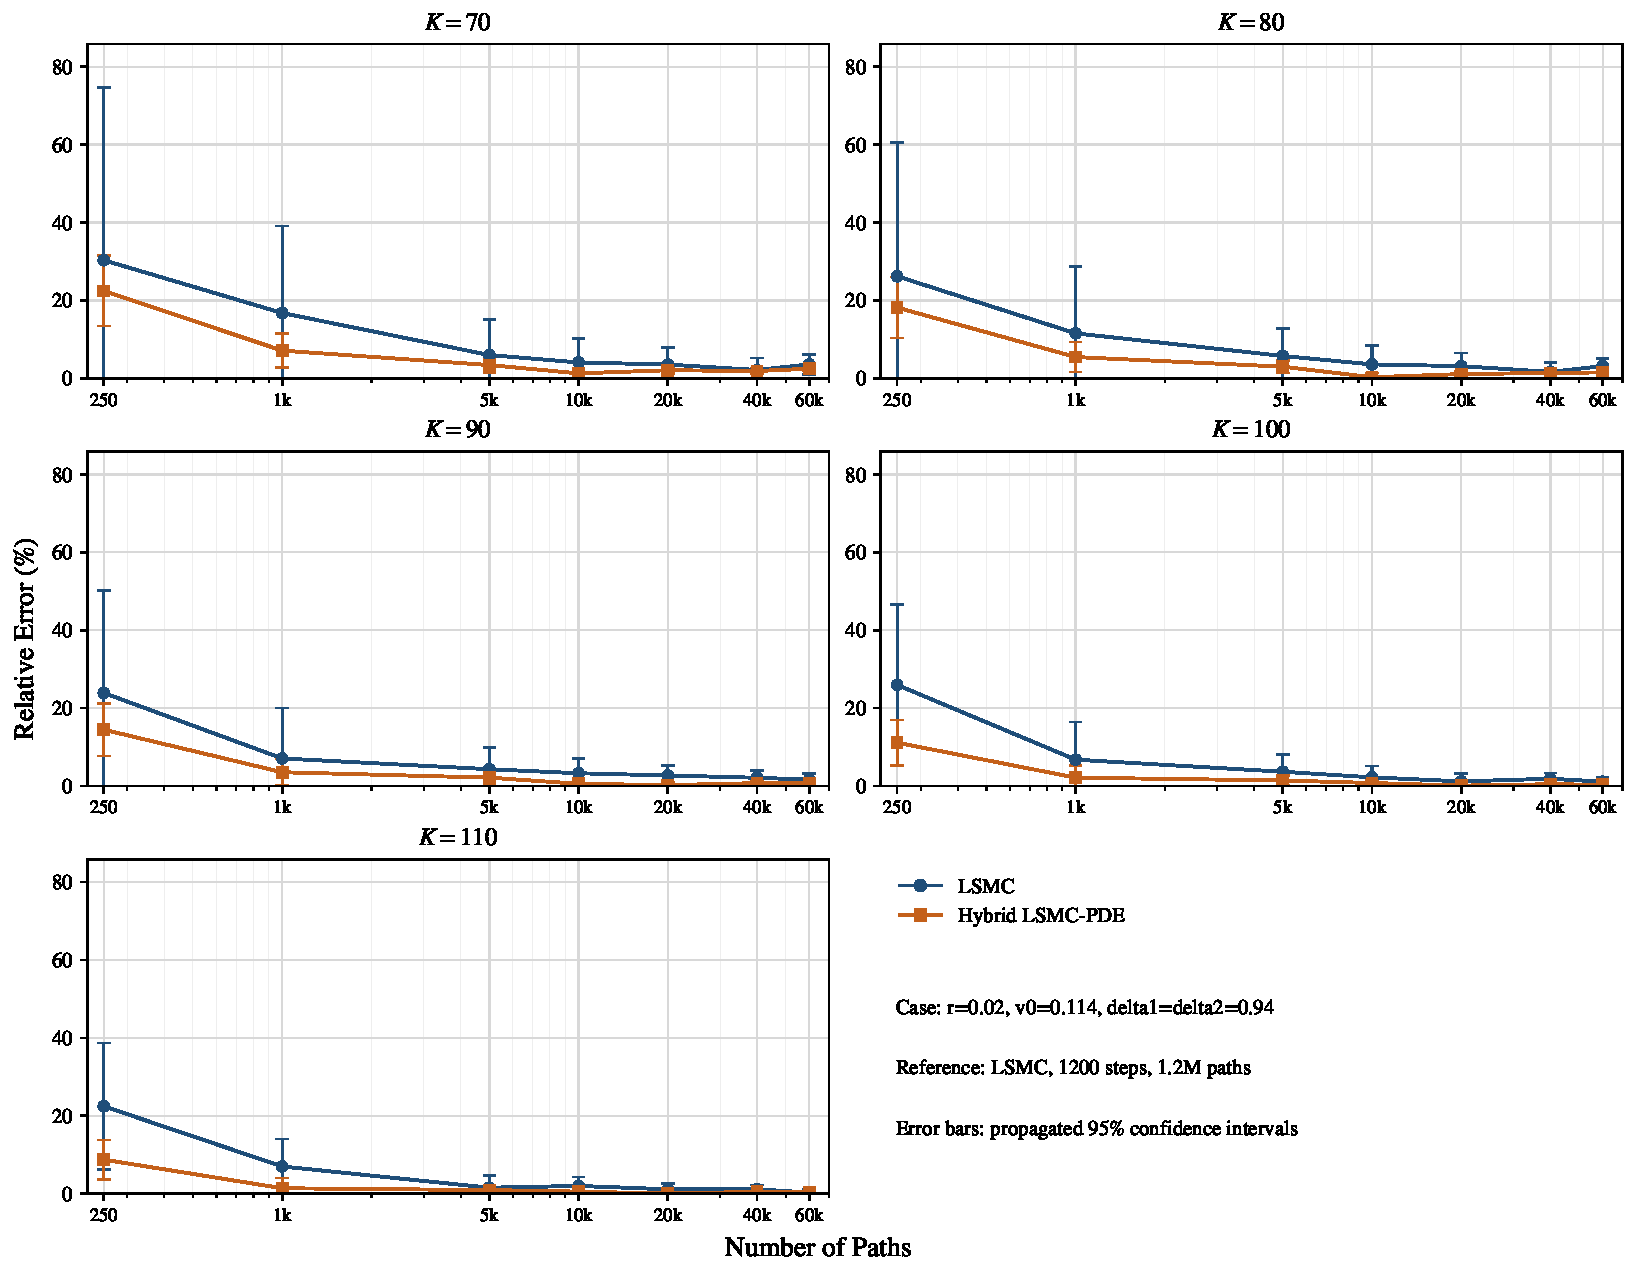
\includegraphics[width=0.96\textwidth]{../figures/bgk_r02_calibrated_t1_nex12_path_sweep_steps48_direct_relative_error.pdf}
\caption{Relative errors for the fixed \(48\)-step path-sweep experiment. Error bars are induced by the \(95\%\) confidence intervals of the direct estimators.}
\label{fig:bgk_r02_calibrated_t1_nex12-path48}
\end{figure}

\begin{table}[htbp]
\centering
\caption{Representative direct metrics at $20{,}000$ paths under the fixed 48-step path sweep.}
\label{tab:bgk_r02_calibrated_t1_nex12-path48-path20k}
\begin{tabular}{lrrrr}
\toprule
Strike & LSMC price & LSMC rel. err. & Hybrid price & Hybrid rel. err. \\
\midrule
$70$ & 2.611646 & 3.520\% & 2.574765 & 2.058\% \\
$80$ & 4.432813 & 3.114\% & 4.345363 & 1.080\% \\
$90$ & 7.129239 & 2.695\% & 6.957089 & 0.216\% \\
$100$ & 10.806834 & 1.168\% & 10.672650 & 0.088\% \\
$110$ & 15.920337 & 1.123\% & 15.746530 & 0.019\% \\
\bottomrule
\end{tabular}
\end{table}


At \(60\) steps for the at-the-money strike, the corresponding LSMC range is 1.324\%--28.932\%, and the Hybrid LSMC--PDE range is 0.049\%--10.102\%. Figure~\ref{fig:bgk_r02_calibrated_t1_nex12-path60} and Table~\ref{tab:bgk_r02_calibrated_t1_nex12-path60-path20k} provide the companion summaries.

\begin{figure}[htbp]
\centering
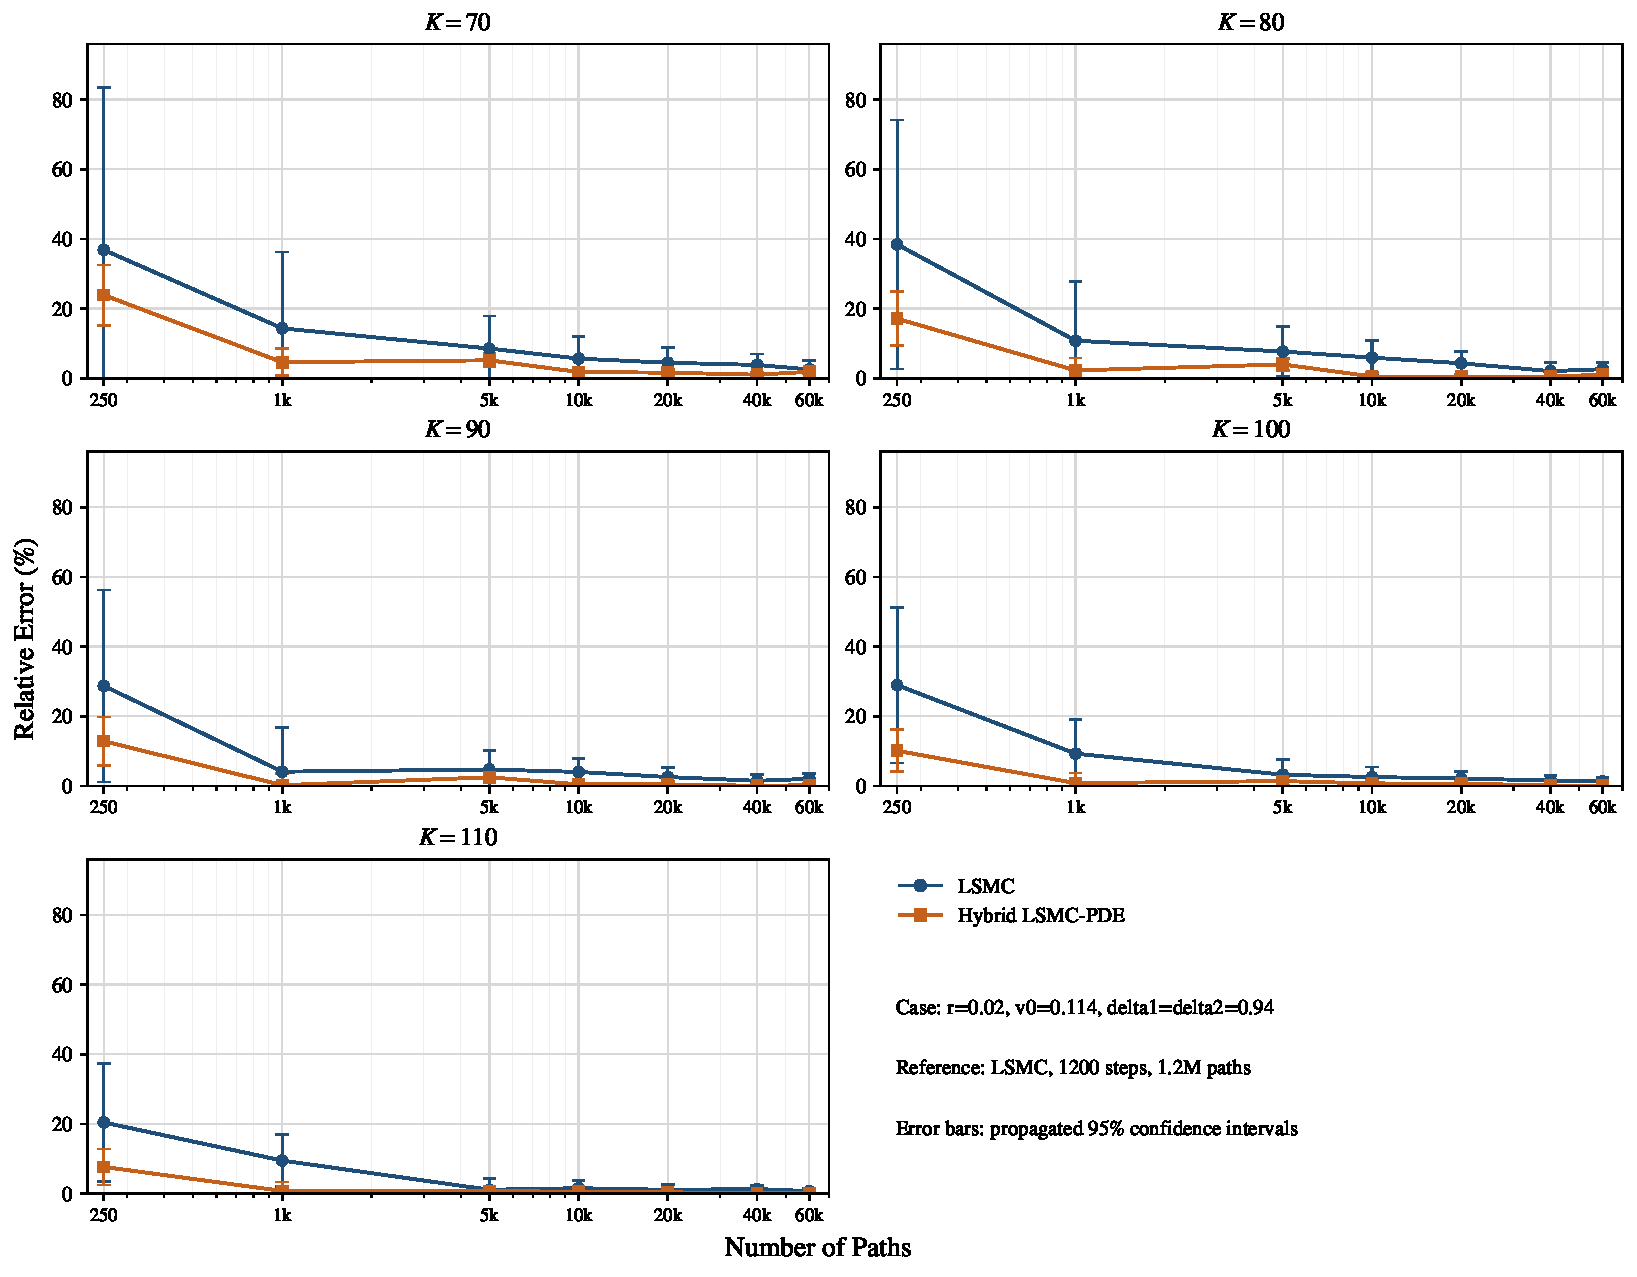
\includegraphics[width=0.96\textwidth]{../figures/bgk_r02_calibrated_t1_nex12_path_sweep_steps60_direct_relative_error.pdf}
\caption{Relative errors for the fixed \(60\)-step path-sweep experiment. Error bars are induced by the \(95\%\) confidence intervals of the direct estimators.}
\label{fig:bgk_r02_calibrated_t1_nex12-path60}
\end{figure}

\begin{table}[htbp]
\centering
\caption{Representative direct metrics at $20{,}000$ paths under the fixed 60-step path sweep.}
\label{tab:bgk_r02_calibrated_t1_nex12-path60-path20k}
\begin{tabular}{lrrrr}
\toprule
Strike & LSMC price & LSMC rel. err. & Hybrid price & Hybrid rel. err. \\
\midrule
$70$ & 2.635093 & 4.449\% & 2.563087 & 1.595\% \\
$80$ & 4.483550 & 4.294\% & 4.317574 & 0.434\% \\
$90$ & 7.119832 & 2.560\% & 6.910022 & 0.462\% \\
$100$ & 10.909701 & 2.131\% & 10.609574 & 0.678\% \\
$110$ & 15.917591 & 1.106\% & 15.679793 & 0.405\% \\
\bottomrule
\end{tabular}
\end{table}


The two experiment families provide a direct check of the pricing behavior under the calibrated positive-rate parameter set. The tables should be read together with the confidence intervals, since both methods retain finite Monte Carlo variability at the moderate path budgets used in the sweeps. The appendix-style tables below list the underlying prices used to form the figures and representative summaries.

\clearpage
\appendix
\section*{Positive-rate gDMR price tables}
\begin{table}[htbp]\centering
\caption{Benchmark prices. Prices are rounded to three decimals.}
\begin{tabular}{lrrrrr}
\toprule
Strike & 70 & 80 & 90 & 100 & 110 \\
\midrule
LSMC benchmark & 2.523 & 4.299 & 6.942 & 10.682 & 15.744 \\
\bottomrule
\end{tabular}
\end{table}

\begin{table}[htbp]\centering
\caption{Fixed-path step-sweep prices with 20,000 paths. Prices are rounded to three decimals.}
\begin{tabular}{lrrrr}
\toprule
Method/step & 24 & 48 & 72 & 96 \\
\midrule
LSMC K=70 & 2.741 & 2.612 & 2.579 & 2.536 \\
Hybrid LSMC-PDE K=70 & 2.711 & 2.575 & 2.547 & 2.565 \\
LSMC K=80 & 4.634 & 4.433 & 4.409 & 4.396 \\
Hybrid LSMC-PDE K=80 & 4.528 & 4.345 & 4.307 & 4.339 \\
LSMC K=90 & 7.341 & 7.129 & 7.068 & 7.080 \\
Hybrid LSMC-PDE K=90 & 7.172 & 6.957 & 6.905 & 6.956 \\
LSMC K=100 & 11.138 & 10.807 & 10.816 & 10.837 \\
Hybrid LSMC-PDE K=100 & 10.898 & 10.673 & 10.607 & 10.679 \\
LSMC K=110 & 16.241 & 15.920 & 15.894 & 15.798 \\
Hybrid LSMC-PDE K=110 & 15.953 & 15.747 & 15.676 & 15.768 \\
\bottomrule
\end{tabular}
\end{table}

\begin{table}[htbp]\centering
\caption{Fixed-path step-sweep prices with 60,000 paths. Prices are rounded to three decimals.}
\begin{tabular}{lrrrr}
\toprule
Method/step & 24 & 48 & 72 & 96 \\
\midrule
LSMC K=70 & 2.718 & 2.612 & 2.579 & 2.533 \\
Hybrid LSMC-PDE K=70 & 2.721 & 2.585 & 2.557 & 2.543 \\
LSMC K=80 & 4.531 & 4.434 & 4.362 & 4.318 \\
Hybrid LSMC-PDE K=80 & 4.547 & 4.364 & 4.326 & 4.307 \\
LSMC K=90 & 7.195 & 7.055 & 7.033 & 6.949 \\
Hybrid LSMC-PDE K=90 & 7.207 & 6.987 & 6.940 & 6.918 \\
LSMC K=100 & 10.996 & 10.800 & 10.794 & 10.712 \\
Hybrid LSMC-PDE K=100 & 10.953 & 10.715 & 10.662 & 10.639 \\
LSMC K=110 & 16.050 & 15.788 & 15.853 & 15.806 \\
Hybrid LSMC-PDE K=110 & 16.026 & 15.803 & 15.749 & 15.725 \\
\bottomrule
\end{tabular}
\end{table}

\begin{table}[htbp]\centering
\caption{Fixed 48-step path-sweep prices. Prices are rounded to three decimals.}
\begin{tabular}{lrrrrrrr}
\toprule
Method/strike & 250 & 1,000 & 5,000 & 10,000 & 20,000 & 40,000 & 60,000 \\
\midrule
LSMC K=70 & 3.288 & 2.946 & 2.673 & 2.625 & 2.612 & 2.576 & 2.612 \\
Hybrid LSMC-PDE K=70 & 3.089 & 2.702 & 2.608 & 2.554 & 2.575 & 2.570 & 2.585 \\
LSMC K=80 & 5.425 & 4.795 & 4.545 & 4.452 & 4.433 & 4.369 & 4.434 \\
Hybrid LSMC-PDE K=80 & 5.079 & 4.533 & 4.427 & 4.310 & 4.345 & 4.357 & 4.364 \\
LSMC K=90 & 8.601 & 7.433 & 7.241 & 7.169 & 7.129 & 7.088 & 7.055 \\
Hybrid LSMC-PDE K=90 & 7.946 & 7.187 & 7.090 & 6.903 & 6.957 & 6.992 & 6.987 \\
LSMC K=100 & 13.454 & 11.404 & 11.072 & 10.918 & 10.807 & 10.881 & 10.800 \\
Hybrid LSMC-PDE K=100 & 11.870 & 10.910 & 10.833 & 10.601 & 10.673 & 10.730 & 10.715 \\
LSMC K=110 & 19.278 & 16.843 & 15.985 & 16.057 & 15.920 & 15.921 & 15.788 \\
Hybrid LSMC-PDE K=110 & 17.120 & 15.962 & 15.889 & 15.660 & 15.747 & 15.819 & 15.803 \\
\bottomrule
\end{tabular}
\end{table}

\begin{table}[htbp]\centering
\caption{Fixed 60-step path-sweep prices. Prices are rounded to three decimals.}
\begin{tabular}{lrrrrrrr}
\toprule
Method/strike & 250 & 1,000 & 5,000 & 10,000 & 20,000 & 40,000 & 60,000 \\
\midrule
LSMC K=70 & 3.452 & 2.884 & 2.738 & 2.665 & 2.635 & 2.619 & 2.587 \\
Hybrid LSMC-PDE K=70 & 3.125 & 2.639 & 2.653 & 2.568 & 2.563 & 2.549 & 2.570 \\
LSMC K=80 & 5.950 & 4.762 & 4.629 & 4.553 & 4.484 & 4.387 & 4.411 \\
Hybrid LSMC-PDE K=80 & 5.034 & 4.396 & 4.470 & 4.321 & 4.318 & 4.321 & 4.342 \\
LSMC K=90 & 8.936 & 7.227 & 7.270 & 7.222 & 7.120 & 7.045 & 7.084 \\
Hybrid LSMC-PDE K=90 & 7.836 & 6.957 & 7.115 & 6.910 & 6.910 & 6.939 & 6.957 \\
LSMC K=100 & 13.773 & 11.673 & 11.026 & 10.955 & 10.910 & 10.850 & 10.823 \\
Hybrid LSMC-PDE K=100 & 11.761 & 10.596 & 10.831 & 10.604 & 10.610 & 10.666 & 10.677 \\
LSMC K=110 & 18.962 & 17.240 & 15.920 & 15.991 & 15.918 & 15.952 & 15.860 \\
Hybrid LSMC-PDE K=110 & 16.953 & 15.621 & 15.863 & 15.659 & 15.680 & 15.755 & 15.757 \\
\bottomrule
\end{tabular}
\end{table}


\end{document}
